\documentclass[a4paper,12pt]{article}
\usepackage[utf8]{inputenc}
\usepackage[spanish]{babel}
\usepackage{color}
\usepackage{parskip}
\usepackage{graphicx}
\usepackage{multirow}
\usepackage{listings}
\usepackage{vmargin}
\graphicspath{ {imagenes/} }
\definecolor{mygreen}{rgb}{0,0.6,0}
\definecolor{lbcolor}{rgb}{0.9,0.9,0.9}
\usepackage{epstopdf}


\setpapersize{A4}
\setmargins{2.5cm}       % margen izquierdo
{1.5cm}                        % margen superior
{16.5cm}                      % anchura del texto
{23.42cm}                    % altura del texto
{10pt}                           % altura de los encabezados
{1cm}                           % espacio entre el texto y los encabezados
{0pt}                             % altura del pie de página
{2cm}     

\lstset{
backgroundcolor=\color{lbcolor},
    tabsize=4,    
%   rulecolor=,
    language=[GNU]C++,
        basicstyle=\tiny,
        aboveskip={1.5\baselineskip},
        columns=fixed,
        showstringspaces=false,
        extendedchars=false,
        breaklines=true,
        prebreak = \raisebox{0ex}[0ex][0ex]{\ensuremath{\hookleftarrow}},
        frame=single,
        showtabs=false,
        showspaces=false,
        showstringspaces=false,
        identifierstyle=\ttfamily,
        keywordstyle=\color[rgb]{0,0,1},
        commentstyle=\color[rgb]{0.026,0.112,0.095},
        stringstyle=\color{red},
        numberstyle=\color[rgb]{0.205, 0.142, 0.73},
%        \lstdefinestyle{C++}{language=C++,style=numbers}’.
}

\begin{document}
  \textbf{Hecho por:} Christofer Fabián Chávez Carazas
  \section{Problema}
    Implementar todos los recorridos de un arbol binario, con sus respectivos inversos.
   \section{Código}
    \subsection{ArbolBinario.h}
      \begin{lstlisting}
#ifndef ARBOLBINARIO_H
#define ARBOLBINARIO_H
#include "iostream"
#include "list"

using namespace std;

class ArbolBinario
{
    public:
        class Nodo{
            public:
            Nodo();
            Nodo(int);
            int valor;
            Nodo * hijos[2];
        };
        ArbolBinario();
        void amplitud();
        void amplitudInverso();
        void insert(int);
        void postorden();
        void preorden();
        void inorden();
        void inordenInverso();
        void postordenInverso();
        void preordenInverso();
        virtual ~ArbolBinario();
    protected:
    private:
        void _postorden(Nodo *&);
        void _inorden(Nodo *&);
        void _preorden(Nodo *&);
        void _inordenInverso(Nodo *&);
        void _postordenInverso(Nodo *&);
        void _preordenInverso(Nodo *&);
        Nodo * root;

};

void ArbolBinario::amplitudInverso(){
    if(!root)return;
    list<Nodo *> result;
    result.push_back(root);
    for(auto iter = result.begin(); iter != result.end(); ++iter){
        if((*iter)->hijos[0]){
            result.push_back((*iter)->hijos[0]);
        }
        if((*iter)->hijos[1]){
            result.push_back((*iter)->hijos[1]);
        }
    }
    for(auto iter = result.begin(); iter != result.end(); ++iter){
        cout<<(*iter)->valor<<endl;
    }
};

void ArbolBinario::preordenInverso(){
    _preordenInverso(root);
}

void ArbolBinario::postordenInverso(){
    _postordenInverso(root);
}
void ArbolBinario::inordenInverso(){
    _inordenInverso(root);
}

void ArbolBinario::_preordenInverso(Nodo *&nodo){
    if(!nodo)return;
    cout<<nodo->valor<<endl;
    _preordenInverso(nodo->hijos[1]);
    _preordenInverso(nodo->hijos[0]);
}

void ArbolBinario::_postordenInverso(Nodo *&nodo){
    if(!nodo)return;
    _postordenInverso(nodo->hijos[1]);
    _postordenInverso(nodo->hijos[0]);
    cout<<nodo->valor<<endl;
}

void ArbolBinario::_inordenInverso(Nodo *&nodo){
    if(!nodo)return;
    _inordenInverso(nodo->hijos[1]);
    cout<<nodo->valor<<endl;
    _inordenInverso(nodo->hijos[0]);
}
void ArbolBinario::amplitud(){
    if(!root)return;
    list<Nodo *> result;
    result.push_back(root);
    for(auto iter = result.begin(); iter != result.end(); ++iter){
        if((*iter)->hijos[0]){
            result.push_back((*iter)->hijos[0]);
        }
        if((*iter)->hijos[1]){
            result.push_back((*iter)->hijos[1]);
        }
    }
    for(auto iter = result.begin(); iter != result.end(); ++iter){
        cout<<(*iter)->valor<<endl;
    }
}

void ArbolBinario::preorden(){
    _preorden(root);
}

void ArbolBinario::inorden(){
    _inorden(root);
}

void ArbolBinario::postorden(){
    _postorden(root);
}

void ArbolBinario::_postorden(Nodo *& nodo){
    if(!nodo)return;
    _postorden(nodo->hijos[0]);
    _postorden(nodo->hijos[1]);
    cout<<nodo->valor<<endl;
}

void ArbolBinario::_inorden(Nodo *& nodo){
    if(!nodo)return;
    _inorden(nodo->hijos[0]);
    cout<<nodo->valor<<endl;
    _inorden(nodo->hijos[1]);
}

void ArbolBinario::_preorden(Nodo *&nodo){
    if(!nodo)return;
    cout<<nodo->valor<<endl;
    _preorden(nodo->hijos[0]);
    _preorden(nodo->hijos[1]);
}

void ArbolBinario::insert(int valor){
    Nodo ** iter = &(root);
    while(*iter){
        iter = &((*iter)->hijos[(*iter)->valor <= valor]);
    }
    *iter = new Nodo(valor);
}

ArbolBinario::Nodo::Nodo(){
    valor = 0;
    hijos[0] = nullptr;
    hijos[1] = nullptr;
}

ArbolBinario::Nodo::Nodo(int valor){
    this->valor = valor;
    hijos[0] = nullptr;
    hijos[1] = nullptr;
}

ArbolBinario::ArbolBinario(){
    root = nullptr;
}

ArbolBinario::~ArbolBinario(){}


#endif // ARBOLBINARIO_H

      \end{lstlisting}

     \subsection{main.h}
     \begin{lstlisting}
#include <iostream>
#include "ArbolBinario.h"

using namespace std;

int main()
{
    ArbolBinario arbolito;
    arbolito.insert(17);
    arbolito.insert(25);
    arbolito.insert(32);
    arbolito.insert(43);
    arbolito.insert(44);
    arbolito.insert(72);
    arbolito.insert(106);
    arbolito.insert(27);
    arbolito.insert(12);
    arbolito.insert(8);
    arbolito.insert(1);
    cout<<"Preorden->"<<endl;
    arbolito.preorden();
    cout<<endl<<"Inorden->"<<endl;
    arbolito.inorden();
    cout<<endl<<"Posorden->"<<endl;
    arbolito.postorden();
    cout<<endl<<"Amplitud->"<<endl;
    arbolito.amplitud();
    cout<<endl<<"Preorden Inverso->"<<endl;
    arbolito.preordenInverso();
    cout<<endl<<"Inorden Inverso->"<<endl;
    arbolito.inordenInverso();
    cout<<endl<<"Posorden Inverso->"<<endl;
    arbolito.postordenInverso();
    cout<<endl<<"Amplitud Inversa->"<<endl;
    arbolito.amplitudInverso();
}

     \end{lstlisting}
  
    \section{Ejemplo}
    \begin{figure}[h]
      \centering
      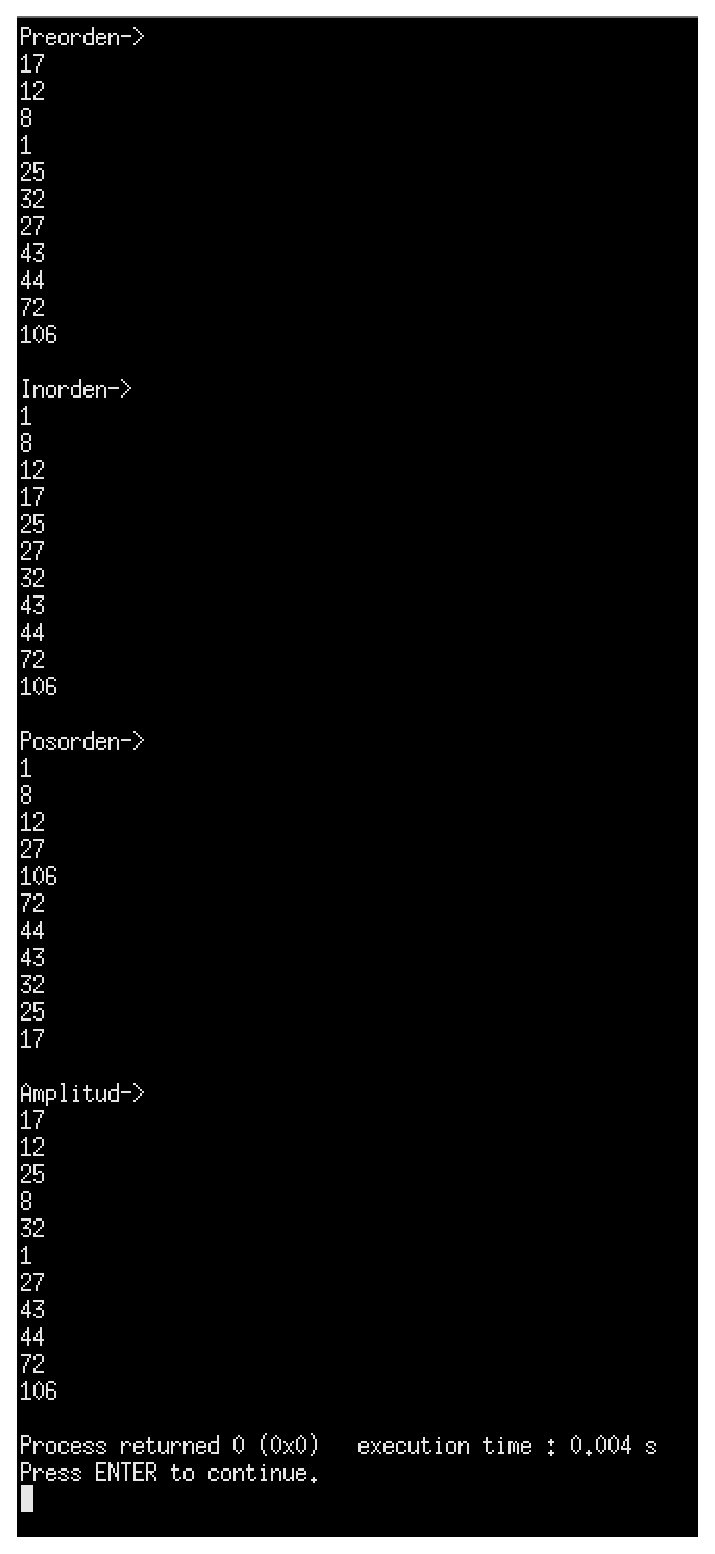
\includegraphics[scale = 0.6]{1.eps}
      \caption{Pruebas part. 1}
    \end{figure}
    \begin{figure}[h]
      \centering
      \includegraphics[scale = 0.6]{2.eps}
      \caption{Pruebas part. 2}
    \end{figure}
\end{document}
